\documentclass{article}
\usepackage{waspaa23}
\usepackage[dvipdfmx]{graphicx}
\usepackage{xcolor}
\usepackage{amsmath}
\usepackage{amsfonts}
\usepackage{url}

\usepackage{cite}
% \usepackage{times}
\usepackage[nolist,nohyperlinks]{acronym}
\usepackage{flushend}

\usepackage{bm}
\usepackage{booktabs}
\usepackage{siunitx}
\usepackage{subcaption}
\usepackage{cleveref}

\usepackage{bsssym}

\title{Rotation Robust Online Independent Vector Analysis with\\Sound Field Interpolation of Circular Microphone Array}
\name{%
  Taishi Nakashima \textsuperscript{\textdagger},
  Yukoh Wakabayashi \textsuperscript{\textdaggerdbl},
  Nobutaka Ono \textsuperscript{\textdagger}
  \thanks{This work was supported by JST CREST Grant Number \mbox{JPMJCR19A3} and JSPS KAKENHI Grant Number \mbox{JP21J22039}, Japan.}
}
\address{%
  \begin{minipage}{.5\textwidth}
    \begin{tabular}{@{}c@{}}
      \textsuperscript{\textdagger}
      Graduate School of Systems Design,\\
      Tokyo Metropolitan University\\
      {\small 6--6, Asahigaoka, Hino-shi, Tokyo 191--0065, Japan}\\
      {\footnotesize \url{nakashima-taishi@ed.tmu.ac.jp}, \url{onono@tmu.ac.jp}}
    \end{tabular}
  \end{minipage}
  \hfill
  \begin{minipage}{.5\textwidth}
    \begin{tabular}{@{}c@{}}
      \textsuperscript{\textdaggerdbl}
      Graduate School of Engineering,\\
      Toyohashi University of Technology\\
      {\small 1--1 Hibarigaoka, Tempaku-cho, Toyohashi, Aichi, 441--8580}\\
      {\footnotesize \url{wakayuko@cs.tut.ac.jp}}
    \end{tabular}
  \end{minipage}
}

\begin{document}
\maketitle

\begin{abstract}
  本論文では,マイクロホンアレイの回転移動に頑健なオンラインブラインド音源分離手法を提案する.
  \begin{itemize}
    \item オンラインIVAはオンライン音源分離に広く用いられている
    \item オンラインIVAは収束が遅い
    \item 身につけるデバイスでオンラインIVAを適用する場合,マイクが短い時間で大きく動きうる
    \item マイクの移動に対してより頑健に分離を行いたい
    \item 先行研究ではビームフォーマで有効性が確認されている
    \item 本研究では音源数が未知の条件で音源分離を行いたい
\end{itemize}
  シミュレーション実験により,音場補間を行うことで音源分離性能が向上したことを確認した.
\end{abstract}
\begin{keywords}
  Blind source separation,
  online source separation,
  independent vector analysis,
  circular microphone array,
  sound field interpolation
\end{keywords}

\section{はじめに}
ブラインド音源分離など多くのアレイ信号処理では,時不変な系を仮定する.
しかし,実応用のためにはマイクロホンや音源の移動など系の時間変化を考慮する必要がある.
そこで,系の時間変化のひとつとして,円状等間隔マイクロホンアレイ(以下,円状アレイ)の回転移動を考え,音場の補間により対応する手法 \cite{Wakabayashi:2020:ASJ:A} が提案された.
この手法は円状アレイの対称性を利用することで,円状アレイが回転する前の音場を簡単な線形演算により推定する.
また,ビームフォーミング \cite{Wakabayashi:2021:ICASSP} やステアリングベクトル推定 \cite{Wakabayashi:2021:ASJ:A} への応用や,
円状アレイの回転角度を自己推定する手法 \cite{Lian:2021:APSIPA} も提案されている.
本稿では,円状アレイが回転する状況下のブラインド音源分離に取り組む.
音場補間により円状アレイの回転移動の影響を打ち消し,後段にブラインド音源分離を適用する.
さらに,シミュレーション実験により音源分離性能を評価する.

\section{問題設定}
音源の数を$\Src$,マイクの数を$\Mic$とする.
短時間フーリエ変換領域において,観測信号$\obs _{\ft} \in \C ^{\Mic}$は
\begin{equation}
  \obs _{\ft} = \sum _{\src=1} ^{\Src} \steer _{\src\ft} \sig _{\src\ft},
\end{equation}
でモデル化されると仮定する.
ただし,
$\freq = 1, \dots, \Freq$は周波数ビンインデクス,
$\tframe = 1, \dots, \Freq$は時間フレームインデクス,
$\sig _{\src\ft} \in \C\; (\src = 1, \dots, \Src)$は$\src$個目の音源信号,
$\steer _{\src\ft} \in \C ^{\Mic}\; (\src = 1, \dots, \Mic)$はそのステアリングベクトルである.

オンラインブラインド音源分離の目的は,現在と過去の観測信号$\{\obs _{\freq,i}\} _{i=1} ^{\tframe}$のみを用いて,
分離行列を推定し,音源を分離することである:
\begin{align}
  \Demix _{\ft} &= \begin{bmatrix} \demix _{1\ft} & \dots & \demix _{\Src\ft} \end{bmatrix} \in \C ^{\Src \times \Mic}, \\
  \est _{\ft} &= \Demix _{\ft} \obs _{\ft} \in \C ^{\Src},
\end{align}
ここで,$\Demix _{\ft}$は分離行列,$\est _{\ft}$は分離信号である.
本研究では,円状アレイが回転する状況を想定して分離行列を推定することを考え,ある時間フレーム$\rotFra$において円状アレイが角度$\rotDeg$回転したとする.
ただし,$\rotFra$および$\rotDeg$は既知とする.

\section{提案手法}
回転後のマイク位置における観測信号$\rotObs _{\ft}\; (\tframe \geq \rotFra)$とし,
ある行列$\rotMat (\rotDeg) \in \C ^{\Mic\times\Mic}$を用いて
\begin{equation}
  \rotObs _{\ft} = \rotMat (\rotDeg) \obs _{\ft}
\end{equation}
と近似する方法が文献 \cite{Wakabayashi:2020:ASJ:A} で示されている.
$\rotObs _{\ft}$の具体的な計算方法は文献 \cite{Wakabayashi:2020:ASJ:A} を見よ.
円状アレイ回転前の時間フレーム$\tframe < \rotFra$における観測信号$\obs _{\ft}$を用いて分離行列$\Demix _{\ft}$が推定できていたとする.
次のように音場補間を適用し,回転前の観測信号を推定することで,円状アレイが回転した後も分離行列を推定し直すことなく分離信号$\est _{\ft}$が得られる.
\begin{equation}
  \est _{\ft} = \Demix _{\ft} \rotObs _{\ft} = \Demix _{\ft} \left(\rotMat (\rotDeg)^{-1} \obs _{\ft}\right).
\end{equation}

本論文では,音源分離手法として
補助関数型独立ベクトル分析 (auxiliary-function-based independent vector analysis; IVA) \cite{Ono:2011:WASPAA}
およびそのオンライン拡張 (OIVA) \cite{Taniguchi:2014:HSCMA} を用いる.
いずれの手法においても,円状アレイの回転を含む観測信号に対して音場補間を適用した後の信号を改めて音源分離の入力とする.

IVAでは,各音源$\src = 1, \dots, \Src$に対して次の更新式で時不変な分離行列$\Demix _{\freq}$を推定する.
\begin{align}
  \srcvar _{\src\tframe} &\gets \sqrt{\textstyle\sum _{\freq} \lvert \demix ^{\hermite} _{\src\ft} \obs ^{\nohermite}_{\ft} \rvert ^2}, \\
  \cov _{\src\ft} &\gets \frac{1}{\Tframe} \sum _{\tframe} \weight (\srcvar_{\src\tframe}) \obs _{\ft} \obs _{\ft}^{\hermite}, \\
  \demix _{\src\ft} &\gets (\Demix _{\ft} \cov _{\src\ft}) ^{-1} \bm{e} _{\src} \label{eq:ip:proj}, \\
  \demix _{\src\ft} &\gets {\demix _{\src\ft}} / {\sqrt{\demix _{\src\ft} ^{\hermite} \cov _{\src\ft} \demix _{\src\ft}}} \label{eq:ip:norm}.
\end{align}
ここで,$\demix _{\src\freq}^{\hermite}$は分離行列の$\src$行目のベクトル,$\Tframe$は時間フレームの総数,$\bm{e}_{\src}$は単位行列の$\src$列目のベクトルである.
$\cov _{\src\freq}$は{重み付き共分散行列}と呼ばれる.
$\weight(\srcvar)$は音源モデルによって定まる関数であり,
本稿では時変Gauss分布$\weight (\srcvar) = \Freq/{\srcvar ^2}$ \cite{Ono:2012:APSIPA}を用いる.

一方,OIVAでは重み付き共分散行列を次のように各時間フレーム$\tframe$ごとに共分散行列を更新し,分離行列を\cref{eq:ip:proj}, \cref{eq:ip:norm}で更新する~\cite{Taniguchi:2014:HSCMA}.
\begin{equation}
  \cov _{\src\ft} \gets \forget \cov _{\src\freq(\tframe-1)} + (1 - \forget) \weight ({\srcvar _{\src\tframe}}) \obs _{\ft} \obs _{\ft}^{\hermite}.
\end{equation}
ここで,$\forget\; (0 \leq \forget < 1)$は忘却係数である.

\subsection{Frequency band limitation}
TBD
\begin{itemize}
  \item 音場補間は周波数が高くなるほどモデルとの乖離が大きくなり補間性能が悪くなる \cite{Wakabayashi:2020:ASJ:A}
  \item 音源分離に用いる音源モデル$\srcvar _{\src\tframe}$を計算するとき,補間がうまくできている周波数帯域だけで計算すれば分離性能が改善されると期待できる
  \item サンプリング周波数$\freqSamp~\unit{\hertz}$,FFT点数$\nfft$のとき,STFTの周波数ビンインデクス$\freq$と物理的な周波数$\freqPhys$の対応
    \begin{equation}
      \freqPhys = \frac{(\freq - 1)\times\freqSamp}{\nfft} \quad \left(\freq = 1, \dots, \frac{\nfft}{2} + 1\right),
    \end{equation}
  \item 修正された音源モデルの更新式
    \begin{equation}
      \srcvar _{\src\tframe} = \sqrt{\sum _{\freq = 1} ^{\SubFreq} \lvert \demix _{\src\ft} \obs _{\ft} \rvert ^2},
    \end{equation}
    ただし,$\SubFreq$は周波数の上限
\end{itemize}

\section{シミュレーション実験}
\subsection{条件}
円状アレイが回転する環境におけるブラインド音源分離の性能を評価する.
音源信号として,SiSECデータベース \cite{Araki:2012:LVAICA}から男性・女性各1サンプル音源を選んだ.
音源信号のサンプリング周波数は\SI{16}{\kilo\hertz}であり,長さ\SI{40}{\second}になるよう加工した.
これらの信号を用いて\cref{fig:room}に示す部屋で鏡像法 \cite{Allen:1979:JASA} によるシミュレーションを行い音像を生成した.
残響時間は約\SI{100}{\milli\second}である.
\begin{figure}[t]
  \centering
  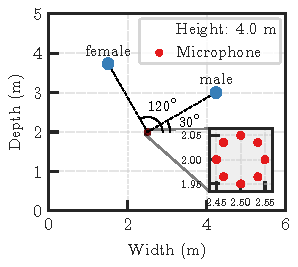
\includegraphics{figures/room_layout.pdf}
  \caption{Room layout.}
  \label{fig:room}
\end{figure}
マイクロホンアレイとしてマイク数$\Mic = 8$,半径\SI{5}{\cm}の円状アレイを用いた.
円状アレイを\cref{fig:room}中の水平軸から反時計周りに0度,30度,45度回転させた場合の音像を生成し,
それぞれ0--10\si{\second},10--25\si{\second},25--40\si{\second}の区間でつなぎ合わせることでマイクロホンアレイの回転を擬似的に再現した.
得られた観測信号に対してフレーム長4096点,シフト長1024点,Hamming窓で短時間フーリエ変換を行い音源分離および音場補間処理を行う.
IVAおよびOIVAの分離行列の初期値は単位行列とした.
反復回数はIVAは100,OIVAは2とした.
OIVAは忘却係数$\forget$を\num{0.97},\num{0.99}および\num{0.995}と変化させながら音源分離を行った.
観測信号に対して音場補間を適用した場合と適用しない場合について音源分離を行い,scale-invariant signal-to-distortion ratio (SI-SDR) \cite{LeRoux:2019:ICASSP} およびその改善量(以下,SDRi)をチャネルごとに平均をとった結果で評価する.
本実験では音場補間によって円状アレイの回転移動を補償した信号に対して音源分離を行うため,SI-SDR, SDRiの計算に用いる参照信号は円状アレイが回転していない場合の音像を用いた.
また,OIVAにおいては,分離信号を\SI{1}{\second}ごとの区間に分割し,各区間でSDRiを計算した.

\subsection{結果}
まず,IVAの結果は
音場補間を適用しないのとき\SI[round-mode=places,round-precision=3]{-5.104996}{\decibel}であり,十分な分離性能が得られていない.
これは,バッチ処理であるIVAを適用しているためマイクアレイの回転に追従できないためと考えられる.
次に,音場補間ありのとき\SI[round-mode=places,round-precision=3]{-1.094806}{\decibel}であった.
前の結果と比較すると改善しているものの,やはり十分な分離性能ではない.
これは音場補間の誤差によるものと考えられる.

次に,OIVAの結果を\cref{fig:online}に示す.
\begin{figure}[t]
  \centering
  \begin{subfigure}[t]{\linewidth}
    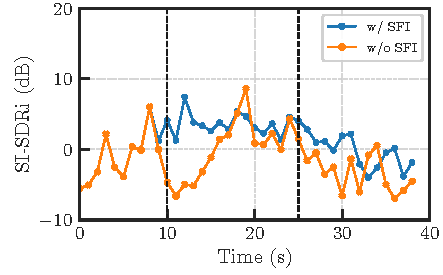
\includegraphics{figures/plots/online/Gauss_8000_97.pdf}
    \caption{$\forget = 0.99$}
  \end{subfigure}
  \begin{subfigure}[t]{\linewidth}
    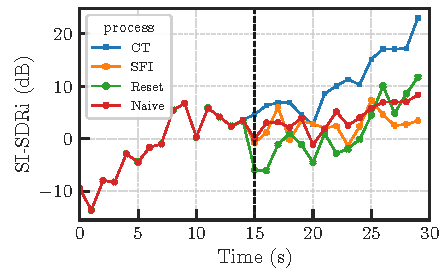
\includegraphics{figures/plots/online/Gauss_8000_99.pdf}
    \caption{$\forget = 0.99$}
  \end{subfigure}
  \begin{subfigure}[t]{\linewidth}
    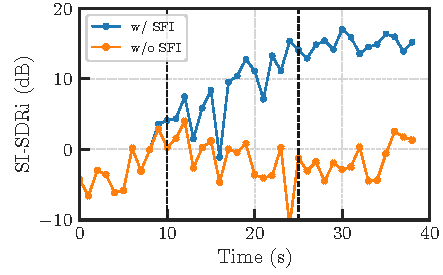
\includegraphics{figures/plots/online/Gauss_8000_995.pdf}
    \caption{$\forget = 0.995$}
  \end{subfigure}
  \caption{Frame-wise SI-SDR improvements (dB). Two vertical dotted lines at \SI{10}{\second} and \SI{25}{\second} denote the rotaion of microphone array.}
  \label{fig:online}
\end{figure}
図中の点線は円状アレイの回転を表す.
まず,忘却係数$\forget=0.97$のとき,音場補間を適用した信号は,\SI{10}{\second}から\SI{25}{\second}の区間でおよそ\SI{5}{\decibel}の分離性能が得られているが,\SI{25}{\second}以降で分離性能が低下した.
忘却係数$\forget=0.99$のとき,前の結果と比較して全体的に分離性能が大きく改善しており,円状アレイの回転にも頑健であることが確認できる.
次に,忘却係数$\forget=0.995$のとき,$\alpha = 0.99$の結果と比べて分離性能の増加が遅くなっているものの,円状アレイの回転後も\SI{10}{\decibel}付近の分離性能を維持できていることがわかる.

\section{おわりに}
本研究では,円状等間隔マイクロホンアレイにおける音場補間をブラインド音源分離に応用した.
シミュレーション実験により,音場補間を行うことで円状等間隔マイクロホンアレイの回転移動する状況でも頑健に音源分離が適用できることを確認した.
今後は本手法の自己回転角度推定 \cite{Lian:2021:APSIPA} との組み合わせや,実時間処理への拡張などに取り組む.

% \section*{Acknowledgments}
% This work was supported by JST CREST Grant Number \mbox{JPMJCR19A3} and JSPS KAKENHI Grant Number \mbox{JP21J22039}, Japan.
\clearpage\newpage
\bibliographystyle{IEEEtran}
\bibliography{IEEEabrv,ref}

\end{document}
